
\chapter{SELKS}
\label{chap:selks}

\definition{SELKS}{SELKS is a free and open source Debian (with LXDE X-window manager) based IDS/IPS platform released under GPLv3 from Stamus Networks (https://www.stamus-networks.com/).\cite{stamusnetworks:_selks}

The SELKS ISO is both Live and Installable ISO in one. Once installed it is ready to use out of the box solution.

SELKS is comprised of the following major components:
\begin{itemize}[itemsep=0pt]
\item[\textbf{S}] Suricata IDPS - http://suricata-ids.org/
\item[\textbf{E}] Elasticsearch - http://www.elasticsearch.org/overview/
\item[\textbf{L}] Logstash - http://www.elasticsearch.org/overview/
\item[\textbf{K}] Kibana - http://www.elasticsearch.org/overview/
\item[\textbf{S}] Scirius - https://github.com/StamusNetworks/scirius
\end{itemize}
}

So SELKS is an OS which contains many softwares. Firstly there is Suricata which is the network analyzer which raise
alerts. Alerts produce by Suricata are written in a EVE file. Then Logstash traduce this file into a JSON file
readable by Elasticsearch. Elasticsearch is a data base. It keep all event and permit a navigation into many
millions of events almost instantaneous. And to finish Kibana propose a User interface for this data base. The
figure \ref{fig:selks_archi} represents this architecture.\footnote{SIEM (security information and event management)
  which are not developed here, are software to analyze and display event of every security tools.}%\footnote{This
%  figure was inspired from the figure 4 in \cite{leblond:suricata}}


You can see on figure \ref{fig:kibana}, an example of the interface of kibana which give an overview of alerts.
This image was extract from the Twitter of Stamus Networks.


\begin{figure}[h]
  \centering
  
\includegraphics[width=0.5\textwidth]{selks_desktop}
  \caption{screenshot of SELKS desktop}
  \label{fig:selks}
\end{figure}

\begin{figure}[h]
  \centering
  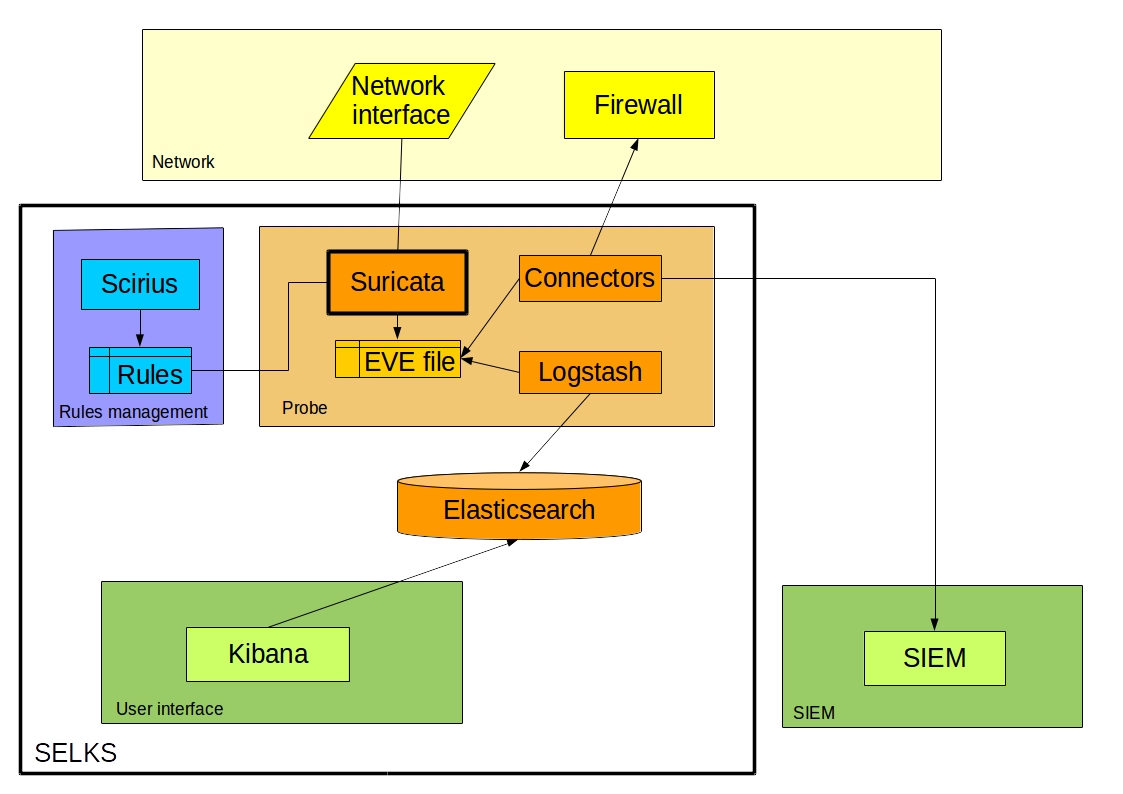
\includegraphics[width=\textwidth]{selks_archi}
  \caption{Selks architecture}
  \label{fig:selks_archi}
\end{figure}



\begin{figure}[h]
  \centering
  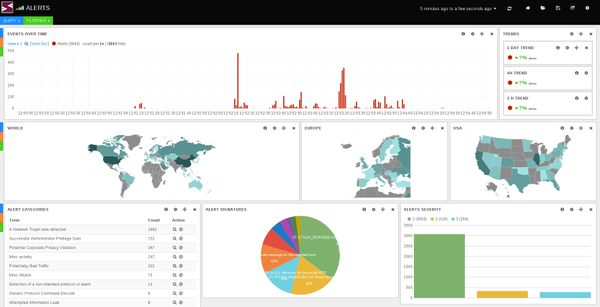
\includegraphics[width=\textwidth]{kibana}
  \caption{Kibana interface}
  \label{fig:kibana}
\end{figure}


%%% Local Variables:
%%% mode: latex
%%% TeX-master: "../rapport_de_base"
%%% End:
